% Created 2022-09-27 Tue 11:07
\documentclass[9pt, b5paper]{article}
\usepackage{xeCJK}
\usepackage{minted}
\usepackage[T1]{fontenc}
\usepackage[scaled]{beraserif}
\usepackage[scaled]{berasans}
\usepackage[scaled]{beramono}
\usepackage{graphicx}
\usepackage{xcolor}
\usepackage{multirow}
\usepackage{multicol}
\usepackage{float}
\usepackage{textcomp}
\usepackage{algorithm}
\usepackage{algorithmic}
\usepackage{latexsym}
\usepackage{natbib}
\usepackage{geometry}
\geometry{left=1.2cm,right=1.2cm,top=1.5cm,bottom=1.2cm}
\newminted{common-lisp}{fontsize=\footnotesize} 
\usepackage[xetex,colorlinks=true,CJKbookmarks=true,linkcolor=blue,urlcolor=blue,menucolor=blue]{hyperref}
\author{deepwaterooo}
\date{\today}
\title{Unity Android SDK/NDK 俄罗斯方块砖3D 小游戏}
\hypersetup{
  pdfkeywords={},
  pdfsubject={},
  pdfcreator={Emacs 27.1 (Org mode 8.2.7c)}}
\begin{document}

\maketitle
\setcounter{tocdepth}{5}
\tableofcontents


\section{模块搭建}
\label{sec-1}
\begin{itemize}
\item \# only inlcude two levels in TOC
\item ILRuntime的消化理解,以及与MVVM同用时的搭配理解消化
\item 热更新模块服务器模块的理解与消化搭建:
\end{itemize}

\section{把原理弄懂}
\label{sec-2}
\begin{itemize}
\item 热更新模块的实充:以前的设计模式和实现的功能还是比较完整的;现在更成熟一点儿,需要把热更新模块补充出来;
\item ILRuntime + MVVM框架设计:两者结合,前几年的时候没能把MVVM理解透彻;
\item 上次前几年主要的难点:好像是在把MVVM双向数据绑定理解得不透彻;那么这次应该就狠没有问题了,更该寻求更好的设计与解决方案
\item 性能优化:另外是对其实高级开发的越来越熟悉,希望应用的性能表现,尤其是渲染性能与速度等、这些更为高级和深入的特性成为这次二次开发的重点。

\item 现在是把自己几年前的写的游戏全忘记了,需要回去把自己的源码找出来,再读一读熟悉一下自己的源码,了解当时设计的估缺点,由此改进更将
\end{itemize}

\section{环境弄得比较好的包括:}
\label{sec-3}
\begin{itemize}
\item 输入法的搭建:终于用到了自己之前用过的好用的输入法
\item 这两天开车疲累,最迟明天中午会去南湾找房间出租,尽快解决搬家的问题;昨天晚上回来得太晚了,一路辛苦,路上只差睡着,回到家里补觉补了好多个小时。
\item 小电脑,笔记本电脑里的游戏环境搭建,今天下午去图书馆里弄(今天下午去图书馆里把需要借助快速网络来完成的事情都搭建好;家里被恶房东故意整了个腾腾慢的网,故意阻碍别人的发展,谁还愿意再这样的环境中继续住下去呢?!!!)
\end{itemize}

\section{ILRuntime 库的系统再深入理解}
\label{sec-4}
\subsection{ILRuntime基本原理}
\label{sec-4-1}
\begin{itemize}
\item ILRuntime借助Mono.Cecil库来读取DLL的PE信息,以及当中类型的所有信息,最终得到方法的IL汇编码,然后通过内置的IL解译执行虚拟机来执行DLL中的代码。IL解释器代码在ILIntepreter.cs,通过Opcode来逐语句执行机器码,解释器的代码有四千多行。
\end{itemize}

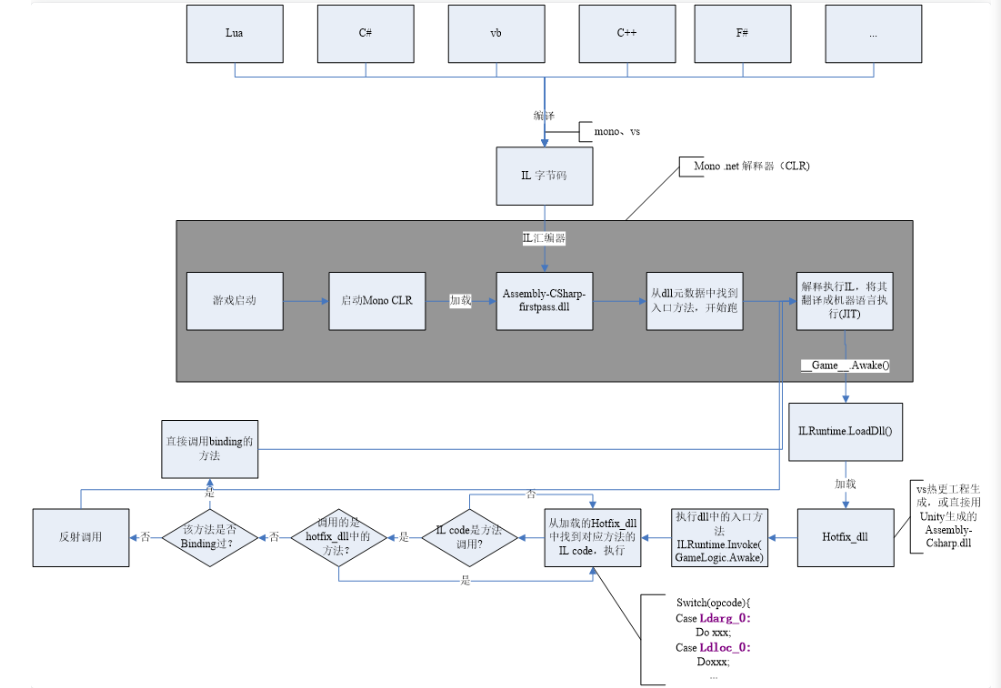
\includegraphics[width=.9\linewidth]{./pic/readme_20220926_094936.png}
\subsection{ILRuntime热更流程}
\label{sec-4-2}

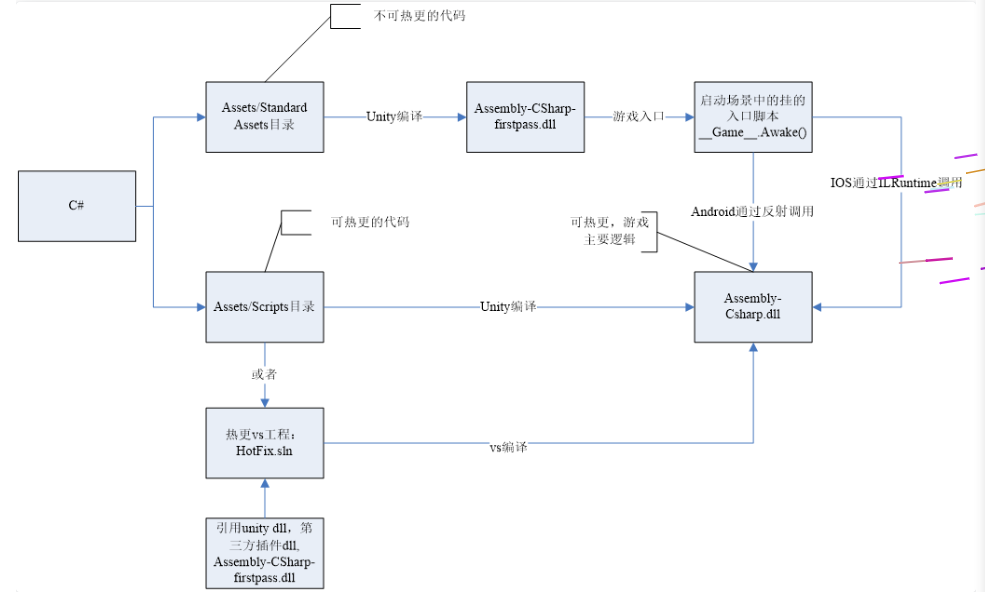
\includegraphics[width=.9\linewidth]{./pic/readme_20220926_095022.png}
\subsection{ILRuntime主要限制}
\label{sec-4-3}

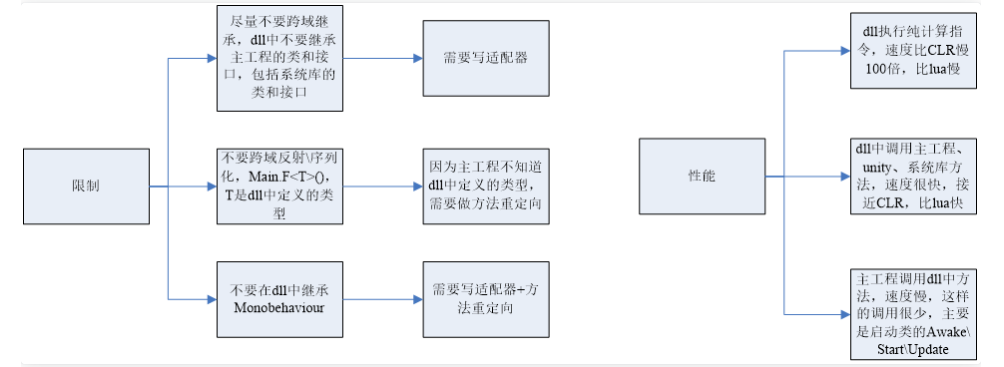
\includegraphics[width=.9\linewidth]{./pic/readme_20220926_095555.png}
\subsection{ILRuntime启动调试}
\label{sec-4-4}
\begin{itemize}
\item ILRuntime建议全局只创建一个AppDomain,在函数入口添加代码启动调试服务
\end{itemize}
\begin{minted}[fontsize=\scriptsize,linenos=false]{csharp}
appdomain.DebugService.StartDebugService(56000)
\end{minted}
\begin{itemize}
\item 运行主工程(Unity工程)
\item 在热更的VS工程中 点击 - 调试 - 附加到ILRuntime调试,注意使用一样的端口
\item 如果使用VS2015的话需要Visual Studio 2015 Update3以上版本
\end{itemize}
\subsection{线上项目和资料}
\label{sec-4-5}
\begin{itemize}
\item 掌趣很多项目都是使用ILRuntime开发,并上线运营,比如:真红之刃,境·界 灵压对决,全民奇迹2,龙族世界,热血足球
\item 初音未来:梦幻歌姬 使用补丁方式:\url{https://github.com/wuxiongbin/XIL}
\item 本文流程图摘自:ILRuntime的QQ群的《ILRuntime热更框架.docx》(by a 704757217)
\item Unity实现c\#热更新方案探究(三): \url{https://zhuanlan.zhihu.com/p/37375372}
\end{itemize}

\section{Framework.MVVM Unity中定义好的MVVM架构}
\label{sec-5}
\subsection{Model}
\label{sec-5-1}
\subsubsection{ModuleBase.cs}
\label{sec-5-1-1}
\begin{minted}[fontsize=\scriptsize,linenos=false]{csharp}
public abstract class ModuleBase {
    public abstract void OnInitialize();
    public abstract void Excute();
}
\end{minted}
\subsubsection{ModuleBaseAdapter : CrossBindingAdaptor:继承了CrossBindingAdaptor这个抽象基类}
\label{sec-5-1-2}
\begin{minted}[fontsize=\scriptsize,linenos=false]{csharp}
public class ModuleBaseAdapter : CrossBindingAdaptor { // 继承了CrossBindingAdaptor抽象基类
    public override Type BaseCLRType { // 继承了CrossBindingAdaptor 抽象基类,就应该需要覆写里面定义过的相关方法,改造成自己需要的样子
        get {
            return typeof(ModuleBase);
        }
    }
    public override Type AdaptorType {
        get {
            return typeof(ModuleBaseAdaptor);
        }
    }
   // 抽象基类 CrossBindingAdaptor里两个方法的定义:
        public abstract Type BaseCLRType { get; }
        // If this Adaptor is capable to impelement multuple interfaces, use this Property, AND BaseCLRType should return null
        public virtual Type[] BaseCLRTypes {
            get {
                return null;
            }
        }
        public abstract Type AdaptorType { get; }

    // 抽象蕨类里的抽象方法:需要实现 
    public override object CreateCLRInstance(ILRuntime.Runtime.Enviorment.AppDomain appdomain, ILTypeInstance instance) {
        return new ModuleBaseAdaptor(appdomain, instance);
    }

    // ModuleBase: Framework.MVVM里定义的基类;CrossBindingAdaptorType是ILRuntime.Runtime.Environment里定义的公共接口类interface
    class ModuleBaseAdaptor : ModuleBase, CrossBindingAdaptorType { // 好久没有写cs代码了,这里看得昏昏乎乎,类里定义类,还是相同的类名,有点儿昏呀?

        ILTypeInstance instance;
        ILRuntime.Runtime.Enviorment.AppDomain appdomain;

// 实现对 ModuleBase里的两个抽象方法的调控掌握
        IMethod _onInitialize;
        bool _onInitializeGot;
        IMethod _excute;
        bool _excuteGot;
        
        public ModuleBaseAdaptor() { }
        public ModuleBaseAdaptor(ILRuntime.Runtime.Enviorment.AppDomain appdomain, ILTypeInstance instance) {
            this.appdomain = appdomain; 
            this.instance = instance;
        }
        
        public ILTypeInstance ILInstance { get { return instance; } }

// 覆写ModuleBase里的两个抽象方法
        public override void OnInitialize() {
            if (!_onInitializeGot) {
                _onInitialize = instance.Type.GetMethod("OnInitialize");
                _onInitializeGot = true;
            }
            if (_onInitialize != null) {
                appdomain.Invoke(_onInitialize, instance, null);
            }
        }
        public override void Excute() {
            if (!_excuteGot) {
                _excute = instance.Type.GetMethod("Excute");
                _excuteGot = true;
            }
            if (_excute != null) {
                appdomain.Invoke(_excute, instance, null);
            }
        }
    }
}
\end{minted}
\subsection{ViewModel}
\label{sec-5-2}
\subsubsection{ViewModelBase.cs}
\label{sec-5-2-1}
\begin{minted}[fontsize=\scriptsize,linenos=false]{csharp}
public class ViewModelBase {
    
    private bool _isInitialize;

    public bool IsRevealInProgress {
        get;
        private set;
    }
    public bool IsRevealed {
        get;
        private set;
    }
    public bool IsHideInProgress {
        get;
        private set;
    }
    public ViewModelBase ParentViewModel {
        get;
        set;
    }

    public virtual void OnStartReveal() {
        IsRevealInProgress = true;
        if (!_isInitialize) {
            OnInitialize();
            _isInitialize = true;
        }
    }
    public virtual void OnFinishReveal() {
        IsRevealInProgress = false;
        IsRevealed = true;
    }
    public virtual void OnStartHide() {
        IsHideInProgress = true;
    }
    public virtual void OnFinishHide() {
        IsHideInProgress = false;
        IsRevealed = false;
    }
    
    public virtual void OnDestory() {}
    protected virtual void OnInitialize() {}
}
\end{minted}
\subsubsection{}
\label{sec-5-2-2}
\subsubsection{}
\label{sec-5-2-3}
\subsection{View}
\label{sec-5-3}
\subsubsection{IView<ViewModelBase>}
\label{sec-5-3-1}
\begin{minted}[fontsize=\scriptsize,linenos=false]{csharp}
public interface IView<ViewModelBase> {
    ViewModelBase BindingContext {
        get;
        set;
    }
    void Reveal(bool immediate = false, Action action = null);
    void Hide(bool immediate = false, Action action = null);
}
\end{minted}
\subsubsection{UnityGuiView: IView<ViewModelBase>, 实现或是覆写基类以及泛型里的各种定义过的方法}
\label{sec-5-3-2}
\begin{minted}[fontsize=\scriptsize,linenos=false]{csharp}
// 继承自抽象基类:便需要实现公用接口类里面所定义的三个接口方法
// 泛型类型是ViewModelBase,便可以实现或是覆写里面定义的各种公用、抽象或是protected方法
public abstract class UnityGuiView : IView<ViewModelBase> { // 仍然是抽象基类:这个类比较重要,明天早上再看一下

private bool _isInitialized; // ViewModelBase 里同共有的

// 自已再定义的两个方法,供实现
    public virtual bool DestoryOnHide {
        get {
            return false;
        }
    }
    public virtual bool IsRoot {
        get {
            return false;
        }
    }

    public static Action SetDownRootIndex;
    public Action CloseOtherRootView;
    protected readonly PropertyBinder<ViewModelBase> binder = new PropertyBinder<ViewModelBase>();
    public readonly BindableProperty<ViewModelBase> viewModelProperty = new BindableProperty<ViewModelBase>();

// 实现了抽象接口类,便需要实现里面的所有定义过的接口方法:公用接口类里定义了这三个方法
    public Action RevealedAction {
        get;
        set;
    }
    public Action HiddenAction {
        get;
        set;
    }
    public ViewModelBase BindingContext { // 实现了抽象接口类,便需要实现里面的所有定义过的接口方法:公用接口类里定义了这三个方法 // <<<<<<<<<< 
        get {
            return viewModelProperty.Value;
        }
        set {
            if (!_isInitialized) {
                OnInitialize();
                _isInitialized = true;
            }
            viewModelProperty.Value = value;
        }
    }
    protected virtual void OnInitialize() { // 辅助帮助抽象方法,可以随每个视图里的不同需求再具体定义
        GameObject = ResourceConstant.Loader.LoadClone(BundleName, AssetName, EAssetBundleUnloadLevel.Never);
        GameObject.AddComponent<CanvasGroup>();
        Transform.SetParent(GameObject.Find("ViewRoot").transform, false);
        viewModelProperty.OnValueChanged += OnBindingContextChanged;
    }
// <<<<<<<<<<<<<<<<<<<< 此公用方法关联四个方法:代理模式的RevealedAction + OnAppear() +  OnReveal() + OnRevealed()
// OnAppear() + OnRevealed(): 两个为公用方法,提供给子视图来继承覆写
    public void Reveal(bool immediate = true, Action action = null) { 
        if (action != null) 
            RevealedAction += action;
        OnAppear();
        OnReveal(immediate);
        OnRevealed();
    }
    public void Hide(bool immediate = true, Action action = null) { // <<<<<<<<<<<<<<<<<<<< 
            if (action != null) 
                HiddenAction += action;
        OnHide(immediate);
        OnHidden();
        OnDisappear();
    }
    public virtual void OnAppear() {
        GameObject.SetActive(true);
    }
    private void OnReveal(bool immediate) {
        BindingContext.OnStartReveal();
        if (immediate) {
            Transform.localScale = Vector3.one;
            CanvasGroup.alpha = 1;
        } else 
            StartAnimatedReveal(); // <<<<<<<<<< 
    }
    public virtual void OnRevealed() {
        BindingContext.OnFinishReveal();
        if (RevealedAction != null) 
            RevealedAction();
        if (IsRoot) {
            if (CloseOtherRootView != null) 
                CloseOtherRootView();
        }
        if (SetDownRootIndex != null) 
            SetDownRootIndex();
    }
    private void OnHide(bool immediate) {
        BindingContext.OnStartHide();
        if (immediate) {
            Transform.localScale = Vector3.zero;
            CanvasGroup.alpha = 0;
        } else 
            StartAnimatedHide();
    }
    public virtual void OnHidden() {
        if (HiddenAction != null) 
            HiddenAction();
    }
    public virtual void OnDisappear() {
        GameObject.SetActive(false);
        BindingContext.OnFinishHide();
        if (DestoryOnHide) 
            UnityEngine.Object.Destroy(GameObject);
    }
// OnInitialize() + OnDestory(): ViewModelBase里定义的抽象方法实现,实现必要的基类逻辑    
    public virtual void OnDestory() {
        if (BindingContext.IsRevealed) 
            Hide(true);
        BindingContext.OnDestory();
        BindingContext = null;
        viewModelProperty.OnValueChanged = null;
    }

// 对于视图中需要使用动画的情况:作出了考虑,定义了可以调用的方法    
    protected virtual void StartAnimatedReveal() {
        CanvasGroup.interactable = false;
        Transform.localScale = Vector3.one;
        //huandong
             //CanvasGroup.DOFade(1, 0.2f).SetDelay(0.2f).OnComplete(() =>
             //{
             //    canvasGroup.interactable = true;
             //});
             }
    protected virtual void StartAnimatedHide() {
        CanvasGroup.interactable = false;
        //canvasGroup.DOFade(0, 0.2f).SetDelay(0.2f).OnComplete(() =>
        //{
        //    transform.localScale = Vector3.zero;
        //    canvasGroup.interactable = true;
        //});
    }
    
// 当有用户行为等导致视图变更的时候,需要调用的对所绑定的ViewModel 的变更
    protected virtual void OnBindingContextChanged(ViewModelBase oldValue, ViewModelBase newValue) {
        binder.UnBind(oldValue);
        binder.Bind(newValue);
    }

    // 主要是针对热更新AB(AssetBundle) 包的处理的相关函数的定义
    public virtual string BundleName {
        get {
            return string.Empty;
        }
    }
    public virtual string AssetName {
        get {
            return string.Empty;
        }
    }
    public virtual string ViewName {
        get {
            return string.Empty;
        }
    }
    public virtual string ViewModelTypeName {
        get {
            return string.Empty;
        }
    }
    public GameObject GameObject {
        get;
        set;
    }
    private Transform _transform;
    public Transform Transform {
        get {
            if (_transform == null) {
                _transform = GameObject.transform;
            }
            return _transform;
        }
    }
    private CanvasGroup _canvasGroup;
    public CanvasGroup CanvasGroup {
        get {
            if (_canvasGroup == null) 
                _canvasGroup = GameObject.GetComponent<CanvasGroup>();
            return _canvasGroup;
        }
    }
}
\end{minted}
\subsubsection{UnityGuiViewAdapter : CrossBindingAdapto: 最鼻祖的实体基类}
\label{sec-5-3-3}
\begin{minted}[fontsize=\scriptsize,linenos=false]{csharp}
public class UnityGuiViewAdapter : CrossBindingAdaptor { // 最鼻祖的实体基类

    // 这里是ModuleBaseAdapter里提供的三个接口方法:这里想一想,为什么要实现ModuleBaseAdapter里所定义的三个方法呢,为什么需要如此桥接?
    public override Type BaseCLRType {
        get {
            return typeof(UnityGuiView);
        }
    }
    public override Type AdaptorType {
        get {
            return typeof(UnityGuiViewAdaptor);
        }
    }
    public override object CreateCLRInstance(ILRuntime.Runtime.Enviorment.AppDomain appdomain, ILTypeInstance instance) {
        return new UnityGuiViewAdaptor(appdomain, instance);
    }
    
    class UnityGuiViewAdaptor : UnityGuiView, CrossBindingAdaptorType { // ILRuntime.Enviorment.CrossBindingAdaptorType
        ILTypeInstance instance;
        ILRuntime.Runtime.Enviorment.AppDomain appdomain;
        object[] param2 = new object[2];

        public UnityGuiViewAdaptor() { }
        public UnityGuiViewAdaptor(ILRuntime.Runtime.Enviorment.AppDomain appdomain, ILTypeInstance instance) {
            this.appdomain = appdomain;
            this.instance = instance;
        }
        public ILTypeInstance ILInstance {
            get { return instance; }
        }

// UnityGuiView里所定义的所有公用方法的基类实现:因为后来的继承类可以覆写,但是也可以要求就请按照基类的实现去执行        
        protected override void OnInitialize() { // 辅助帮助抽象方法,可以随每个视图里的不同需求再具体定义
            if (!_onInitializeGot) {
                _onInitialize = instance.Type.GetMethod("OnInitialize");
                _onInitializeGot = true;
            }
            if (_onInitialize != null && !isOnInitializeInvoking) {
                isOnInitializeInvoking = true;
                appdomain.Invoke(_onInitialize, instance);
                isOnInitializeInvoking = false;
            } else 
                base.OnInitialize();
        }
        public override void OnAppear() {
            if (!_onAppearGot) {
                _onAppear = instance.Type.GetMethod("OnAppear");
                _onAppearGot = true;
            }
            if (_onAppear != null && !isOnAppearInvoking) {
                isOnAppearInvoking = true;
                appdomain.Invoke(_onAppear, instance);
                isOnAppearInvoking = false;
            } else {
                base.OnAppear();
            }
        }
        public override void OnRevealed() {
            if (!_onRevealedGot) {
                _onRevealed = instance.Type.GetMethod("OnRevealed");
                _onRevealedGot = true;
            }
            if (_onRevealed != null && !isOnRevealedInvoking) {
                isOnRevealedInvoking = true;
                appdomain.Invoke(_onRevealed, instance);
                isOnRevealedInvoking = false;
            } else {
                base.OnRevealed();
            }
        }
        public override void OnHidden() {
            if (!_onHiddenGot) {
                _onHidden = instance.Type.GetMethod("OnHidden");
                _onHiddenGot = true;
            }
            if (_onHidden != null && !isOnHiddenInvoking) {
                isOnHiddenInvoking = true;
                appdomain.Invoke(_onHidden, instance);
                isOnHiddenInvoking = false;
            } else {
                base.OnHidden();
            }
        }
        public override void OnDisappear() {
            if (!_onDisappearGot) {
                _onDisappear = instance.Type.GetMethod("OnDisappear");
                _onDisappearGot = true;
            }
            if (_onDisappear != null && !isOnDisappearInvoking) {
                isOnDisappearInvoking = true;
                appdomain.Invoke(_onDisappear, instance);
                isOnDisappearInvoking = false;
            } else {
                base.OnDisappear();
            }
        }
        public override void OnDestory() {
            if (!_onDestoryGot) {
                _onDestory = instance.Type.GetMethod("OnDestory");
                _onDestoryGot = true;
            }
            if (_onDestory != null && !isOnDestoryInvoking) {
                isOnDestoryInvoking = true;
                appdomain.Invoke(_onDestory, instance);
                isOnDestoryInvoking = false;
            } else {
                base.OnDestory();
            }
        }
        protected override void StartAnimatedReveal() {
            if (!_startAnimatedRevealGot) {
                _startAnimatedReveal = instance.Type.GetMethod("StartAnimatedReveal");
                _startAnimatedRevealGot = true;
            }
            if (_startAnimatedReveal != null && !isStartAnimatedRevealInvoking) {
                isStartAnimatedRevealInvoking = true;
                appdomain.Invoke(_startAnimatedReveal, instance);
                isStartAnimatedRevealInvoking = false;
            } else {
                base.StartAnimatedReveal();
            }
        }
        protected override void StartAnimatedHide() {
            if (!_startAnimatedHideGot) {
                _startAnimatedHide = instance.Type.GetMethod("StartAnimatedHide");
                _startAnimatedHideGot = true;
            }
            if (_startAnimatedHide != null && !isStartAnimatedHideInvoking) {
                isStartAnimatedHideInvoking = true;
                appdomain.Invoke(_startAnimatedHide, instance);
                isStartAnimatedHideInvoking = false;
            } else {
                base.StartAnimatedHide();
            }
        }
        protected override void OnBindingContextChanged(ViewModelBase oldValue, ViewModelBase newValue) {
            if (!_onBindingContextChangedGot) {
                _onBindingContextChanged = instance.Type.GetMethod("OnBindingContextChanged");
                _onBindingContextChangedGot = true;
            }
            if (_onBindingContextChanged != null && !isOnBindingContextChangedInvoking) {
                isOnBindingContextChangedInvoking = true;
                appdomain.Invoke(_onBindingContextChanged, instance, param2);
                isOnBindingContextChangedInvoking = false;
            } else {
                base.OnBindingContextChanged(oldValue, newValue);
            }
        }

// 下面是处理热更新AB包相关的回调接口控制公用方法:定义为基类实现,因为此类为第一个实体的基类
        public override string BundleName {
            get {
                if (!_getBundleNameGot) {
                    _getBundleName = instance.Type.GetMethod("get_BundleName", 0);
                    _getBundleNameGot = true;
                }
                if (_getBundleName != null && !isGetBundleNameInvoking) {
                    isGetBundleNameInvoking = true;
                    var res = (string)appdomain.Invoke(_getBundleName, instance, null);
                    isGetBundleNameInvoking = false;
                    return res;
                } else {
                    return base.BundleName;
                }
            }
        }
        public override string AssetName {
            get {
                if (!_getAssetNameGot) {
                    _getAssetName = instance.Type.GetMethod("get_AssetName", 0);
                    _getAssetNameGot = true;
                }
                if (_getAssetName != null && !isGetAssetNameInvoking) {
                    isGetAssetNameInvoking = true;
                    var res = (string)appdomain.Invoke(_getAssetName, instance, null);
                    isGetAssetNameInvoking = false;
                    return res;
                } else {
                    return base.AssetName;
                }
            }
        }
        public override string ViewName {
            get {
                if (!_getViewNameGot) {
                    _getViewName = instance.Type.GetMethod("get_ViewName", 0);
                    _getViewNameGot = true;
                }
                if (_getViewName != null && !isGetViewNameInvoking) {
                    isGetViewNameInvoking = true;
                    var res = (string)appdomain.Invoke(_getViewName, instance, null);
                    isGetViewNameInvoking = false;
                    return res;
                } else {
                    return base.ViewName;
                }
            }
        }
        public override string ViewModelTypeName {
            get {
                if (!_getViewModelTypeNameGot) {
                    _getViewModelTypeName = instance.Type.GetMethod("get_ViewModelTypeName", 0);
                    _getViewModelTypeNameGot = true;
                }
                if (_getViewModelTypeName != null && !isGetViewModelTypeNameInvoking) {
                    isGetViewModelTypeNameInvoking = true;
                    var res = (string)appdomain.Invoke(_getViewModelTypeName, instance, null);
                    isGetViewModelTypeNameInvoking = false;
                    return res;
                } else {
                    return base.ViewModelTypeName;
                }
            }
        }

// 覆写UnityGuiView里定义的两个公用抽象方法        
        public override bool DestoryOnHide {
            get {
                if (!_getDestoryOnHideGot) {
                    _getDestoryOnHide = instance.Type.GetMethod("get_DestoryOnHide", 0);
                    _getDestoryOnHideGot = true;
                }
                if (_getDestoryOnHide != null && !isGetDestoryOnHideInvoking) {
                    isGetDestoryOnHideInvoking = true;
                    var res = (bool)appdomain.Invoke(_getDestoryOnHide, instance, null);
                    isGetDestoryOnHideInvoking = false;
                    return res;
                } else {
                    return base.DestoryOnHide;
                }
            }
        }
        public override bool IsRoot {
            get {
                if (!_getIsRootGot) {
                    _getIsRoot = instance.Type.GetMethod("get_IsRoot", 0);
                    _getIsRootGot = true;
                }
                if (_getIsRoot != null && !isGetIsRootInvoking) {
                    isGetIsRootInvoking = true;
                    var res = (bool)appdomain.Invoke(_getIsRoot, instance, null);
                    isGetIsRootInvoking = false;
                    return res;
                } else {
                    return base.IsRoot;
                }
            }
        }
    }
    
// 每个标记变量对应的三小变量    
    IMethod _onInitialize;
    bool _onInitializeGot;
    bool isOnInitializeInvoking = false;

    IMethod _onAppear;
    bool _onAppearGot;
    bool isOnAppearInvoking = false;
    IMethod _onRevealed;
    bool _onRevealedGot;
    bool isOnRevealedInvoking = false;
    IMethod _onHidden;
    bool _onHiddenGot;
    bool isOnHiddenInvoking = false;
    IMethod _onDisappear;
    bool _onDisappearGot;
    bool isOnDisappearInvoking = false;
    IMethod _onDestory;
    bool _onDestoryGot;
    bool isOnDestoryInvoking = false;
    IMethod _startAnimatedReveal;
    bool _startAnimatedRevealGot;
    bool isStartAnimatedRevealInvoking = false;
    IMethod _startAnimatedHide;
    bool _startAnimatedHideGot;
    bool isStartAnimatedHideInvoking = false;
    IMethod _getBundleName;
    bool _getBundleNameGot;
    bool isGetBundleNameInvoking = false;
    IMethod _getAssetName;
    bool _getAssetNameGot;
    bool isGetAssetNameInvoking = false;
    IMethod _getViewName;
    bool _getViewNameGot;
    bool isGetViewNameInvoking = false;
    IMethod _getDestoryOnHide;
    bool _getDestoryOnHideGot;
    bool isGetDestoryOnHideInvoking = false;
    IMethod _getIsRoot;
    bool _getIsRootGot;
    bool isGetIsRootInvoking = false;
    IMethod _getViewModelTypeName;
    bool _getViewModelTypeNameGot;
    bool isGetViewModelTypeNameInvoking = false;
    IMethod _onBindingContextChanged;
    bool _onBindingContextChangedGot;
    bool isOnBindingContextChangedInvoking = false;
}
\end{minted}
\section{HotFix中使用MVVM架构实现热更新的搭配与相关的链接}
\label{sec-6}
% Emacs 27.1 (Org mode 8.2.7c)
\end{document}